\documentclass[11pt,a4paper]{article}  % Déclare la classe du document.

\newcommand{\chaptermark}[2]{\og #2 \fg{} (#1)} % ligne uniquement pour éviter une erreur en cas d'article
\usepackage[table,dvipsnames,svgnames]{xcolor}
\usepackage{listingsutf8}
%\usepackage[utf8]{inputenc}% gestion des accents (source)
\usepackage[T1]{fontenc}% gestion des accents (PDF)
\usepackage{fontspec}
\usepackage[french]{babel}% gestion du français
\usepackage{textcomp}% caractères additionnels
\usepackage{mathtools,amssymb,amsthm}% packages de l'AMS + mathtools
\usepackage{amsmath}
\usepackage{yhmath}
\usepackage{mathpazo}
\usepackage[scaled=0.95]{helvet}
\usepackage{courier}
%\usepackage{fourier}
%\usepackage[scaled=0.95]{helvet}
%\usepackage{courier}
\usepackage{bm}
\usepackage{gensymb}
\usepackage{graphicx}

\usepackage{enumitem}
\usepackage{pifont}

\usepackage{pstricks}
\usepackage{pstricks-add}
\usepackage{pst-eucl}
\usepackage{pgfplots}
\let\clipbox\relax
%\usepackage{pst-plot,pst-text,pst-tree,pstricks-add}
%\usepackage{pst-node} % required package
\usepackage{pst-all}
\usepackage[most,skins,breakable]{tcolorbox}

\usepackage{euscript}





% ############### Nouvelles commandes ###############
% Coloration des labels des points dans pst-eucl
\makeatletter
\define@key[psset]{pst-eucl}{LabelColor}{\def\psk@LabelColor{#1}}
\psset{LabelColor=black}
\def\Pst@WhichLabel#1{{\color{\psk@LabelColor}%
		\ifx\psk@PointName\@default#1\else\psk@PointName\fi}}
\makeatother

% renomme le symbole #2 en #1#2 et invalide le symbole initial #2:
\def\renamesymbol#1#2{
	\expandafter\let\expandafter\newsym\expandafter=\csname#2\endcsname
	\expandafter\global\expandafter\let\csname#1#2\endcsname=\newsym
	\expandafter\global\expandafter\let\csname#2\endcsname=\origsym
}



\usepackage{ProfCollege}
\renamesymbol{Casio}{Calculatrice}
\usepackage[nonshellescape]{ProfLycee}



%\usepackage[left=1.5cm,right=1.5cm,top=2.5cm,bottom=2.5cm]{geometry}
\usepackage[left=13mm,right=13mm,top=18mm,bottom=18mm,footskip=30pt]{geometry}
\setlength{\headheight}{15pt}

\usepackage{titlesec}
\usepackage{pas-math}
\usepackage{longtable}
\usepackage{tikz,tkz-tab}
\usepackage{amsmath}
\usepackage[right]{eurosym}
\usepackage{sectsty}
\usepackage{tipfr}
\usepackage{setspace}

%pour faire les touches de la calculatrices
\usepackage{menukeys}
\renewmenumacro{\menu}{roundedmenus} % default: menus
\renewmenumacro{\directory}{pathswithfolder} % default: paths
\renewmenumacro{\keys}{shadowedroundedkeys} % default: roundedkeys


\usepackage{multicol}
\usepackage{multirow}
\usepackage{systeme}

%% Format des titres de chapitres, paragraphes, ...
\titleformat{\chapter}[frame]
{\color{red!85!white}\normalsize}%
{\filright\sffamily\Large%
	\enspace Chapitre \thechapter\enspace}%
{8pt}
{\color{red!85!white}\rule{0pt}{30pt}\sffamily\Huge\bfseries\filcenter}
%%%%%%%%%%%%%%%%%%%%
\titlespacing{\chapter}{0pc}{0pc}{2pc}
\titlespacing{\subsection}{2pc}{}{}

\titleformat{\subsection}[block]{\hspace{1em}}{\thesubsection}{1em .}{}
\titleformat{\subsubsection}[block]{\hspace{2em}}{\thesubsection}{1em )}{}

\chapterfont{\color{red}{}}
\sectionfont{\color{green!55!black}{}}
\subsectionfont{\color{cyan!65!black}{}}
\subsubsectionfont{\color{violet}{}}
\renewcommand{\thesection}{\color{green!55!black}\Roman{section}.}
\renewcommand{\thesubsection}{\color{cyan!65!black}\arabic{subsection})}
\renewcommand{\thesubsubsection}{\color{violet}\alph{subsubsection})}
\setcounter{secnumdepth}{3}

\titleformat{\subsection}[block]{\hspace{1em}}{\thesubsection}{1em .}{}
\titleformat{\subsubsection}[block]{\hspace{2em}}{\thesubsection}{1em )}{}

\usepackage[column=A]{cellspace}
\setlength{\cellspacebottomlimit}{4pt}
\setlength{\cellspacetoplimit}{4pt}
\setlength{\parindent}{2pt}
\setlength{\tabcolsep}{0.5cm}


%entête et pieds de pages
\usepackage{fancyhdr}
\pagestyle{fancy}
\fancyhf{}
\usepackage{lastpage}
\renewcommand{\chaptermark}[1]{\markboth {Chap. \thechapter~ - ~#1}{}}
\renewcommand\headrulewidth{1pt}
\fancyhead[LO,RE]{1ère G - spécialité maths}
\fancyhead[RO,LE]{\leftmark}
\renewcommand\footrulewidth{1pt}
\fancyfoot[LO,RE]{Année 2025-2026}
\fancyfoot[RO,LE]{\textbf{Page \thepage/\pageref{LastPage}}}

%Mes boites pour les définitions, propriétés, remarques, ...

%Mes boites pour les définitions, propriétés, remarques, ...

\newcommand\titrebox[1]{\textbf{#1}}
\newtcolorbox{definition}{breakable,colback=red!10!white,
	colframe=red!85!white, fonttitle=\bfseries,enhanced,
	attach boxed title to top left={xshift=5mm, yshift=-2mm},boxed title style={size=small,colback=red!10!white,colframe=red!85!white, arc=0.5mm},
	title=\textcolor{red!85!white}{Définition} , arc=3mm}

\newtcolorbox{definitionTitre}[1]{breakable,colback=red!10!white,
	colframe=red!85!white, fonttitle=\bfseries,enhanced,
	attach boxed title to top left={xshift=5mm, yshift=-2mm},boxed title style={size=small,colback=red!10!white,colframe=red!85!white, arc=0.5mm},
	title=\textcolor{red!85!white}{Définition - #1} , arc=3mm}

\newtcolorbox{definitionPerso}[1]{breakable,colback=red!10!white,
	colframe=red!85!white, fonttitle=\bfseries,enhanced,
	attach boxed title to top left={xshift=5mm, yshift=-2mm},boxed title style={size=small,colback=red!10!white,colframe=red!85!white, arc=0.5mm},
	title=\textcolor{red!85!white}{#1} , arc=3mm}

\newtcolorbox{regle}{breakable,colback=red!10!white,
	colframe=red!85!white, fonttitle=\bfseries,enhanced,
	attach boxed title to top left={xshift=5mm, yshift=-2mm},boxed title style={size=small,colback=red!10!white,colframe=red!85!white, arc=0.5mm},
	title=\textcolor{red!85!white}{Règle} , arc=3mm}

\newtcolorbox{regles}{breakable,colback=red!10!white,
	colframe=red!85!white, fonttitle=\bfseries,enhanced,
	attach boxed title to top left={xshift=5mm, yshift=-2mm},boxed title style={size=small,colback=red!10!white,colframe=red!85!white, arc=0.5mm},
	title=\textcolor{red!85!white}{Règles} , arc=3mm}

\newtcolorbox{definitions}{breakable,colback=red!10!white,
	colframe=red!85!white, fonttitle=\bfseries,enhanced,
	attach boxed title to top left={xshift=5mm, yshift=-2mm},boxed title style={size=small,colback=red!10!white,colframe=red!85!white, arc=0.5mm},
	title=\textcolor{red!85!white}{Définitions} , arc=3mm}

\newtcolorbox{propriete}{breakable,colback=red!10!white,
	colframe=red!85!white, fonttitle=\bfseries,enhanced,
	attach boxed title to top left={xshift=5mm, yshift=-2mm},boxed title style={size=small,colback=red!10!white,colframe=red!85!white, arc=0.5mm},
	title=\textcolor{red!85!white}{Propriété} , arc=3mm}

\newtcolorbox{proprieteTitre}[1]{breakable,colback=red!10!white,
	colframe=red!85!white, fonttitle=\bfseries,enhanced,
	attach boxed title to top left={xshift=5mm, yshift=-2mm},boxed title style={size=small,colback=red!10!white,colframe=red!85!white, arc=0.5mm},
	title=\textcolor{red!85!white}{Propriété - #1} , arc=3mm}

\newtcolorbox{proprietes}{breakable,colback=red!10!white,
	colframe=red!85!white, fonttitle=\bfseries,enhanced,
	attach boxed title to top left={xshift=5mm, yshift=-2mm},boxed title style={size=small,colback=red!10!white,colframe=red!85!white, arc=0.5mm},
	title=\textcolor{red!85!white}{Propriétés} , arc=3mm}

\newtcolorbox{theoreme}{breakable,colback=red!10!white,
	colframe=red!85!white, fonttitle=\bfseries,enhanced,
	attach boxed title to top left={xshift=5mm, yshift=-2mm},boxed title style={size=small,colback=red!10!white,colframe=red!85!white, arc=0.5mm},
	title=\textcolor{red!85!white}{Théorème} , arc=3mm}

\newtcolorbox{theoremeTitre}[1]{breakable,colback=red!10!white,
	colframe=red!85!white, fonttitle=\bfseries,enhanced,
	attach boxed title to top left={xshift=5mm, yshift=-2mm},boxed title style={size=small,colback=red!10!white,colframe=red!85!white, arc=0.5mm},
	title=\textcolor{red!85!white}{Théorème - #1} , arc=3mm}

\newtcolorbox{theoremes}{breakable,colback=red!10!white,
	colframe=red!85!white, fonttitle=\bfseries,enhanced,
	attach boxed title to top left={xshift=5mm, yshift=-2mm},boxed title style={size=small,colback=red!10!white,colframe=red!85!white, arc=0.5mm},
	title=\textcolor{red!85!white}{Théorèmes} , arc=3mm}

\newtcolorbox{bexemple}{
	enhanced,
	breakable,
	fonttitle=\bfseries,
	frame empty,
	nobeforeafter,
	borderline west={0.5mm}{0mm}{cyan!75!black},
	title=\textcolor{cyan!75!black}{\faHubspot\:\:Exemple},
	%title after break=Exemple (suite),
	colback=white,
	extras={enhanced, frame empty},
	detach title,before upper={\tcbtitle\ :\quad },
}

\newtcolorbox{bexemples}{
	enhanced,
	breakable,
	fonttitle=\bfseries,
	frame empty,
	nobeforeafter,
	borderline west={0.5mm}{0mm}{cyan!75!black},
	title=\textcolor{cyan!75!black}{\faHubspot\:\:Exemples},
	%title after break=Exemples (suite),
	colback=white,
	extras={enhanced, frame empty},
	detach title,before upper={\tcbtitle\ :\quad },
}

\newtcolorbox{bexemplet}[1]{
	enhanced,
	breakable,
	fonttitle=\bfseries,
	frame empty,
	borderline west={0.5mm}{0mm}{cyan!75!black},
	title=\textcolor{cyan!75!black}{\faHubspot\:\:Exemple - #1},
	colback=white,
	extras={enhanced, frame empty},
	detach title,before upper={\tcbtitle\ :\quad },
}

\newtcolorbox{brmq}{
	enhanced,
	breakable,
	fonttitle=\bfseries,
	frame empty,
	nobeforeafter,
	borderline west={0.5mm}{0mm}{orange!95!white},
	title=\textcolor{orange!85!white}{\faHandPointRight[regular]\:\:Remarque} ,
	colback=white,
	extras={enhanced, frame empty},
	detach title,before upper={\tcbtitle\ \quad },
}

\newtcolorbox{brmqs}{
	enhanced,
	breakable,
	fonttitle=\bfseries,
	frame empty,
	nobeforeafter,
	borderline west={0.5mm}{0mm}{orange!85!white},
	title=\textcolor{orange!85!white}{\faHandPointRight[regular]\:\:Remarques},
	colback=white,
	detach title,before upper={\tcbtitle\ \quad },
	extras={enhanced, frame empty},
}

\newtcolorbox{brmqt}[1]{
	enhanced,
	breakable,
	fonttitle=\bfseries,
	frame empty,
	nobeforeafter,
	borderline west={0.5mm}{0mm}{orange!85!white},
	title=\textcolor{orange!85!white}{\faHandPointRight[regular]\:\:Remarque - #1},
	colback=white,
	extras={enhanced, frame empty},
	detach title,before upper={\tcbtitle\ \quad },
}

\newtcolorbox{consequences}[1]{
	enhanced,
	breakable,
	fonttitle=\bfseries,
	frame empty,
	nobeforeafter,
	borderline west={0.5mm}{0mm}{ProcessBlue},
	title=\textcolor{ProcessBlue}{#1},
	colback=white,
	extras={enhanced, frame empty},
	detach title,before upper={\tcbtitle\ :\quad },
}

\newtcolorbox{bmethode}{
	enhanced,
	breakable,
	fonttitle=\bfseries,
	frame empty,
	nobeforeafter,
	borderline west={0.5mm}{0mm}{blue!75!black},
	title=\textcolor{blue!75!black}{Méthode} ,
	colback=white,
	extras={enhanced, frame empty},
	attach boxed title to top left = {xshift = -3mm},
	boxed title style={size=small,colback=white,colframe=blue!75!black, arc=3mm,
	}
}

\newtcolorbox{bmethodes}{
	enhanced,
	breakable,
	fonttitle=\bfseries,
	frame empty,
	nobeforeafter,
	borderline west={0.5mm}{0mm}{blue!75!black},
	title=\textcolor{blue!75!black}{Méthodes} ,
	colback=white,
	extras={enhanced, frame empty},
	attach boxed title to top left = {xshift = -3mm},
	boxed title style={size=small,colback=blue!75!black,colframe=blue!75!black, arc=3mm,
	}
	boxed title after break style={size=small,colback=white,colframe=blue!75!black, arc=3mm,
	}
}

\newtcolorbox{bmethodet}[1]{
	enhanced,
	breakable,
	fonttitle=\bfseries,
	frame empty,
	nobeforeafter,
	borderline west={0.5mm}{0mm}{blue!75!black},
	title=\textcolor{blue!75!black}{\faTasks\:\:Méthode - #1} ,
	colback=white,
	extras={enhanced, frame empty},
	attach boxed title to top left = {xshift = -3mm},
	boxed title style={size=small,colback=white,colframe=blue!75!black, arc=3mm,
	}
}

\newtcolorbox{bdemo}{
	enhanced,
	breakable,
	fonttitle=\bfseries,
	frame empty,
	nobeforeafter,
	borderline west={0.5mm}{0mm}{violet!65!white},
	title={\faEdit[regular]\:\:Démonstration},
	%title after break=Démonstration (suite),
	colback=white,
	extras={enhanced, frame empty},
	attach boxed title to top left = {xshift = -3mm},
	boxed title style={size=small,colback=violet!65!white,colframe=violet!65!white, arc=3mm,
	}
}

\newtcolorbox{bdemos}{
	enhanced,
	breakable,
	fonttitle=\bfseries,
	frame empty,
	nobeforeafter,
	borderline west={0.5mm}{0mm}{violet!65!white},
	title={\faEdit[regular]\:\:Démonstrations},
	%title after break=Démonstration (suite),
	colback=white,
	extras={enhanced, frame empty},
	attach boxed title to top left = {xshift = -3mm},
	boxed title style={size=small,colback=violet!65!white,colframe=violet!65!white, arc=3mm,
	}
}

\newtcolorbox{bdemot}[1]{
	enhanced,
	breakable,
	fonttitle=\bfseries,
	frame empty,
	nobeforeafter,
	borderline west={0.5mm}{0mm}{violet!65!white},
	title={\faEdit[regular]\:\:Démonstration - #1},
	%title after break=Démonstration (suite),
	colback=white,
	extras={enhanced, frame empty},
	attach boxed title to top left = {xshift = -3mm},
	boxed title style={size=small,colback=violet!65!white,colframe=violet!65!white, arc=3mm,
	}
}

\newtcolorbox{boxPerso}[2]{
	enhanced,
	breakable,
	fonttitle=\bfseries,
	frame empty,
	nobeforeafter,
	borderline west={0.5mm}{0mm}{#2},
	title=#1,
	%title after break=Exemple (suite),
	colback=white,
	extras={enhanced, frame empty},
	detach title,before upper={\tcbtitle\ :\quad },
}


\newcommand*{\Coord}[3]{% 
	\ensuremath{\vv{#1}\, 
		\begin{pmatrix} 
			#2\\ 
			#3 
\end{pmatrix}}}

\newcommand*{\CoordSV}[2]{% 
	\ensuremath{\begin{pmatrix} 
			#1\\ 
			#2 
\end{pmatrix}}}

\newcommand*{\Coordp}[3]{% 
	\ensuremath{\vv{#1}\, 
		\left\lvert 
		\begin{matrix} 
			#2\\ 
			#3 
		\end{matrix}  
		\right.% Ne pas oublier le délimiteur invisible. 
}}


%personnalisation des listes non numérotées pour les différentes boites 
\newlist{itemEx}{itemize}{2}
\setlist[itemEx,1]{label=$\bullet$, font=\color{cyan!75!black}}
\setlist[itemEx,2]{label=$\bullet$, font=\color{cyan!75!black}}

\newlist{enumEx}{enumerate}{2}
\setlist[enumEx,1]{label=\arabic*), font=\bf\color{cyan!75!black}}
\setlist[enumEx,2]{label=\alph*), font=\bf\color{cyan!75!black}}

\newlist{itemMet}{itemize}{2}
\setlist[itemMet,1]{label=$\bullet$, font=\color{blue!75!black}}
\setlist[itemMet,2]{label=$\bullet$, font=\color{blue!75!black}}

\newlist{enumMet}{enumerate}{2}
\setlist[enumMet,1]{label=\arabic*), font=\bf\color{blue!75!black}}
\setlist[enumMet,2]{label=\alph*), font=\bf\color{blue!75!black}}

\newlist{itemDef}{itemize}{2}
\setlist[itemDef,1]{label=$\bullet$, font=\color{ForestGreen}}
\setlist[itemDef,2]{label=$\bullet$, font=\color{ForestGreen}}

\newlist{enumDef}{enumerate}{2}
\setlist[enumDef,1]{label=\arabic*), font=\bf\color{ForestGreen}}
\setlist[enumDef,2]{label=\alph*), font=\bf\color{ForestGreen}}

\newlist{itemProp}{itemize}{2}
\setlist[itemProp,1]{label=$\bullet$, font=\color{red!85!white}}
\setlist[itemProp,2]{label=$\bullet$, font=\color{red!85!white}}

\newlist{enumProp}{enumerate}{2}
\setlist[enumProp,1]{label=\arabic*), font=\bf\color{red!85!white}}
\setlist[enumProp,2]{label=\alph*), font=\bf\color{red!85!white}}

\newlist{itemDem}{itemize}{2}
\setlist[itemDem,1]{label=$\bullet$, font=\color{violet!85!white}}
\setlist[itemDem,2]{label=$\bullet$, font=\color{violet!85!white}}

\newlist{enumDem}{enumerate}{2}
\setlist[enumDem,1]{label=\arabic*), font=\bf\color{violet!85!white}}
\setlist[enumDem,2]{label=\alph*), font=\bf\color{violet!85!white}}

\newlist{itemRem}{itemize}{2}
\setlist[itemRem,1]{label=\ding{43}, font=\color{orange!85!white}}
\setlist[itemRem,2]{label=\ding{43}, font=\color{orange!85!white}}

\newlist{enumRem}{enumerate}{2}
\setlist[enumRem,1]{label=\arabic*), font=\bf\color{orange!85!white}}
\setlist[enumRem,2]{label=\alph*), font=\bf\color{orange!85!white}}

% nouvelle commande pour mettre entre guillemets une expression
\newcommand{\guillemets}[1]{\og \emph{#1} \fg}


\newcommand{\corr}[1]{\fcolorbox{red}{yellow!30}{#1}}

\newtcolorbox{corrBox}{enhanced,breakable,boxrule=1pt,nobeforeafter,boxsep=0pt,left=\fboxsep,right=\fboxsep,colback=yellow!30,colframe=red!75!black}

% commandes pour mettre en couleur (et en gras) dans une expression mathématique.
\newcommand{\mVert}[1]{{\color{green!55!black}\bm{#1}}}
\newcommand{\mVertWB}[1]{{\color{green!55!black}#1}}
\newcommand{\mRouge}[1]{{\color{red!85!white}\bm{#1}}}
\newcommand{\mRougeWB}[1]{{\color{red!85!white}#1}}
\newcommand{\mBleu}[1]{{\color{blue!75!black}\bm{#1}}}
\newcommand{\mBleuWB}[1]{{\color{blue!75!black}#1}}
\newcommand{\mOrange}[1]{{\color{orange!75!white}\bm{#1}}}
\newcommand{\mOrangeWB}[1]{{\color{orange!75!white}#1}}
\newcommand{\mViolet}[1]{{\color{violet!85!white}\bm{#1}}}
\newcommand{\mVioletWB}[1]{{\color{violet!85!white}#1}}

%commandes pour les flèches de distributivité.
\newcommand{\tikzmarkBB}[2][]{ \tikz[remember picture, overlay, baseline=-0.5ex]\node[#1, left](#2){}; }
\newcommand{\flechePropV}[4][]{ \tikz[remember picture, overlay]\draw (#2)edge[bend left=90,min distance=1em, -stealth]node[midway, #1]{#4}(#3); }
\newcommand{\flechePropH}[4][]{ \tikz[remember picture, overlay]\draw (#2)edge[bend left=90, min distance=1em, -stealth]node[midway, #1]{#4}(#3); }
\newcommand{\flechePropHbas}[4][]{ \tikz[remember picture, overlay]\draw (#2)edge[bend left=-90, min distance=1em, -stealth]node[midway, #1]{#4}(#3); }


\lstdefinestyle{algo}{%
	inputencoding=utf8,
	mathescape,
	basicstyle=\footnotesize\ttfamily,
	numberstyle=\scriptsize\ttfamily\color{gray},
	showstringspaces=false,
	tabsize=2,
	numbers=left,
	framexleftmargin=8mm,
	xleftmargin=8mm,
	keepspaces=true,
	frame=lines,
	framerule=1pt,
	rulecolor=\color{green!50!black},
	backgroundcolor=\color{green!5},
	keywords = {Pour, allant, Si, alors, Sinon, Fin},    
	morecomment=[l][commentstyle]{//},
	commentstyle=\color{gray},
	classoffset=0,
	keywordstyle=\color{blue!75},
	classoffset=1,
	morekeywords = {Afficher},
	keywordstyle=\color{green!50!black},
	classoffset=0,
	morestring=[b]",
	stringstyle=\color{red!75},
	literate=
	{é}{{\'e}}{1}%
	{è}{{\`e}}{1}%
	{à}{{\`a}}{1}%
	{â}{{\^a}}{1}%%%
	{ç}{{\c{c}}}{1}%
	{œ}{{\oe}}{1}%
	{ù}{{\`u}}{1}%
	{É}{{\'E}}{1}%
	{È}{{\`E}}{1}%
	{À}{{\`A}}{1}%
	{Ç}{{\c{C}}}{1}%
	{Œ}{{\OE}}{1}%
	{Ê}{{\^E}}{1}%
	{ê}{{\^e}}{1}%
	{î}{{\^i}}{1}%
	{ï}{{\"i}}{1}%%%
	{ô}{{\^o}}{1}%
	{û}{{\^u}}{1}%
	{=}{$\leftarrow$}{1}%
	{==}{$={}$}{1}}


%  --------   Macro pour les exercices et leur numérotation  

\newcounter{exo}

\setcounter{exo}{1}

\newcommand{\exercice}[1]{\vskip 0.2cm\noindent{\bf \ Exercice \theexo {  #1 }}\addtocounter{exo}{1}}

\newcounter{rit}

\setcounter{rit}{1}

\newcommand{\rituel}[1]{\vskip 0.2cm\noindent{ \bf \ \underline{Rit. \therit {  #1 }}}\addtocounter{rit}{1}}

\newcommand{\raisedrule}[2][0em]{\leaders\hbox{\rule[#1]{1pt}{#2}}\hfill}

\newcounter{numexo}

\setcounter{numexo}{1}

\newcommand{\exerciceDS}[1]{\vskip 0.6cm\noindent\rule[+2pt]{1cm}{0.5pt}\ {\large\bf \ Exercice \thenumexo {  #1 }}\raisedrule[+2pt]{0.5pt}\null\addtocounter{numexo}{1}\par\vskip 0,4cm}

\newcommand{\bareme}[1]{\tikz\node[circle,draw,inner sep=1pt,outer sep=1pt, color=red]{\textbf{#1}};}

%  --------   Pour le langage Python

% Default fixed font does not support bold face
\DeclareFixedFont{\ttb}{T1}{txtt}{bx}{n}{12} % for bold
\DeclareFixedFont{\ttm}{T1}{txtt}{m}{n}{12}  % for normal

% Custom colors
\usepackage{color}
\definecolor{deepblue}{rgb}{0,0,0.5}
\definecolor{deepred}{rgb}{0.6,0,0}
\definecolor{deepgreen}{rgb}{0,0.5,0}

\usepackage{listings}

% Python style for highlighting
\newcommand\pythonstyle{\lstset{
		language=Python,
		basicstyle=\ttm,
		otherkeywords={self},             % Add keywords here
		keywordstyle=\ttb\color{deepblue},
		emph={MyClass,__init__},          % Custom highlighting
		emphstyle=\ttb\color{deepred},    % Custom highlighting style
		stringstyle=\color{deepgreen},
		frame=tb,                         % Any extra options here
		showstringspaces=false            % 
}}


% Python environment
\lstnewenvironment{python}[1][]
{
	\pythonstyle
	\lstset{#1}
}
{}

% Python for external files
\newcommand\pythonexternal[2][]{{
		\pythonstyle
		\lstinputlisting[#1]{#2}}}

% Python for inline
\newcommand\pythoninline[1]{{\pythonstyle\lstinline!#1!}}


% \begin{document}
	
	% \section{``In-text'' listing highlighting}
	
	% \begin{python}
		% class MyClass(Yourclass):
		%     def __init__(self, my, yours):
		%         bla = '5 1 2 3 4'
		%         print bla
		% \end{python}
	
	% \section{External listing highlighting}
	
	% \pythonexternal{demo.py}
	
	% \section{Inline highlighting}
	
	% Definition \pythoninline{class MyClass} means \dots
	
	% \end{document}

\definecolor{codegreen}{rgb}{0,0.6,0}
\definecolor{codegray}{rgb}{0.5,0.5,0.5}
\definecolor{codepurple}{rgb}{0.58,0,0.82}
\definecolor{backcolour}{rgb}{0.95,0.95,0.92}

\lstdefinestyle{myStyle}{
	backgroundcolor=\color{backcolour},   
	commentstyle=\color{codegreen},
	keywordstyle=\color{magenta},
	numberstyle=\tiny\color{codegray},
	stringstyle=\color{codepurple},
	basicstyle=\ttfamily\footnotesize,
	breakatwhitespace=false,         
	breaklines=true,                 
	captionpos=b,                    
	keepspaces=true,                 
	numbers=left,                    
	numbersep=5pt,                  
	showspaces=false,                
	showstringspaces=false,
	showtabs=false,                  
	tabsize=2
}

\lstset{style=myStyle}

\newcommand{\normeB}[1]{\left\Vert \vv{#1}\right\Vert}

\newcommand\grasmaths[1]{\symbf{#1}}
\newcommand\sfbmath[1]{\symbf{\symsfup{#1}}}
\definecolor{marron}{rgb}{0.64,0.16,0.16}
\definecolor{titrebleu}{rgb}{0,0,0.6}

\usepackage{tabularx}
\usepackage{wasysym}
% ===========================tableaux de base
\newcolumntype{R}[1]{>{\raggedleft\arraybackslash }b{#1}} 
\newcolumntype{L}[1]{>{\raggedright\arraybackslash }b{#1}}
\newcolumntype{C}[1]{>{\centering\arraybackslash }b{#1}}
\newcolumntype{M}[1]{>{\centering\arraybackslash }m{#1}} %doublecentrée
\renewcommand{\tabularxcolumn}[1]{m{#1}}
\newcolumntype{Y}{>{\centering\arraybackslash }X}

%=============================boîtes de cours
\usepackage{fontawesome5}
\newcommand\fontbox{\sffamily}
%\newcommand\titrebox[1]{\textbf{#1}}
\tcbuselibrary{breakable}
\tcbset{bdefaut/.style={%
		fonttitle=\fontbox,%
		enhanced,breakable,center,boxrule=1.25pt,drop shadow=black!33!white,%
		sharp corners=uphill,arc=12pt,before skip=12pt,after skip=12pt,%
		left=5pt,leftupper=5pt,top=1mm,bottom=1mm,%
		before upper=\leavevmode
	}
}
\NewDocumentCommand\bbnewbox{ m m m m O{#4} !O{} }{%nom + titre + icone + bordure/titre/fondtitre + couleur fond + options
	\DeclareTColorBox{#1}{ O{} }{%
		bdefaut,%
		colframe=#4,coltitle=#4!25!Black,colbacktitle=#4!35,colback=#5!10,%
		title={#3\:\:\titrebox{#2##1}},%
		#6
	}%
}

\bbnewbox{bdefi}{Définition}{\faIcon[regular]{comment-dots}}{ForestGreen}
\bbnewbox{bcor}{Corollaire}{\faIcon[regular]{comment-dots}}{ForestGreen}
\bbnewbox{bdefis}{Définitions}{\faIcon[regular]{comment-dots}}{ForestGreen}
\bbnewbox{bhumour}{Humour}{\faIcon[regular]{laugh-wink}}{Yellow}
%\bbnewbox{bprop}{Propriété}{\faCog}{Salmon}
\bbnewbox{bprop}{Propriété}{\faCog}{red!85!white}
\bbnewbox{bprops}{Propriétés}{\faCog}{Salmon}
\bbnewbox{bcscq}{Conséquence}{\faArrowAltCircleRight[regular]}{Salmon}
\bbnewbox{bthm}{Théorème}{\faBullhorn}{FireBrick}
\bbnewbox{blog}{Logiciel}{\faDev}{CornflowerBlue}[white]
\bbnewbox{bhistoire}{Point histoire}{\faUniversity}{Chocolate}[white]

%\bbnewbox{brmq}{Remarque}{\faHandPointRight[regular]}{MidnightBlue}[white]
\bbnewbox{bexercice}{Exercice}{\faHubspot}{MidnightBlue}
%\bbnewbox{bexemple}{Exemple}{\faHubspot}{MediumTurquoise}
\bbnewbox{bvoc}{Vocabulaire}{\faList*[regular]}{YellowGreen}
\bbnewbox{bnota}{Notation}{\faList*}{YellowGreen}
\bbnewbox{bregle}{Règle}{\faList*}{YellowGreen}
\bbnewbox{bcadre}{Cadre}{\faInfoCircle}{Peru}
\bbnewbox{bidee}{Idée}{\faInfo}{LightBlue}
\bbnewbox{bintro}{Intro}{\faMarker}{LightSalmon}
\bbnewbox{billustr}{Illustration}{\faChartLine}{Crimson}[White]
\bbnewbox{bvideo}{}{\faIcon[regular]{file-video}}{teal}[White]
\bbnewbox{bbilan}{Bilan}{\faForward}{Purple}
%\bbnewbox{bmethode}{Méthode}{\faTasks}{Coral}
%\bbnewbox{bmethode}{Méthode}{\faTasks}{blue!75!black}
\bbnewbox{btuto}{Tuto}{\faTerminal}{Coral}[White]
\bbnewbox{bmanip}{Manipulation}{\faCodeBranch}{DarkCyan}[White]
\bbnewbox{bcalco}{Calculatrice}{\faCalculator}{MediumVioletRed}[White]
\bbnewbox{boutil}{Outil}{\faTools}{DeepSkyBlue}[White]
\bbnewbox{basavoir}{À savoir}{\faHeart}{Red}
\bbnewbox{bbloctd}{TD}{\faHourglassStart}{LightSeaGreen}[White]
\bbnewbox{bblocdm}{À vous de jouer}{\faHourglassStart}{LightSeaGreen}[White]
%\bbnewbox{brappel}{Rappel}{\faHandPointUp[regular]}{LightSalmon}
\bbnewbox{brappel}{Rappel}{\faHandPointUp[regular]}{Peru}
\bbnewbox{bresol}{Résolution}{\faPuzzlePiece}{LightSeaGreen}[White]
\bbnewbox{battention}{Attention}{\faExclamationTriangle}{Red}
\bbnewbox{bcode}{Code}{\faCode}{Crimson}[White]
\bbnewbox{bpython}{Python}{\faPython}{SeaGreen}[White]

\newcommand{\grasInDef}[1]{\textcolor{ForestGreen!55!black}{\textbf{#1}}}
\newcommand{\grasInProp}[1]{\textcolor{red!85!white}{\textbf{#1}}}
\newcommand{\grasInEx}[1]{\textcolor{MediumTurquoise!55!black}{\textbf{#1}}}
\newcommand{\grasInRem}[1]{\textcolor{orange!65!white}{\textbf{#1}}}
\newcommand{\grasInMet}[1]{\textcolor{blue!75!black}{\textbf{#1}}}
\newcommand{\grasInDem}[1]{\textcolor{violet!85!white}{\textbf{#1}}}

%\newtcolorbox{bmethodet}[1][]{%
%	bdefaut,%
%	colframe=blue!75!black,coltitle=white,colbacktitle=blue!65!black,colback=blue!75!black!15!white,
%	title={\faTasks\:\:\titrebox{{Méthode - #1}}}
%}

%outil
\newtcolorbox{boutilcalc}[1][]{%
	bdefaut,%
	colframe=DeepSkyBlue,coltitle=black,colbacktitle=DeepSkyBlue!35,colback=White,
	title=\textcolor{DeepSkyBlue!25!Black}{\faFileVideo[regular]\:\:\titrebox{Tuto#1 Vidéo}}
}

%loglogo
\newtcolorbox{bloglogo}[2][]{%
	bdefaut,%
	colframe=CornflowerBlue,coltitle=black,colbacktitle=CornflowerBlue!35,colback=white,
	title=\textcolor{CornflowerBlue!25!Black}{\faDev\:\:\titrebox{Logiciel#1}},
	overlay={\begin{tcbclipinterior}
			\node[opacity=0.33,rotate=-45] at ($(interior.south east)+(-10pt,10pt)$){\includegraphics[height=24pt]{#2}};
	\end{tcbclipinterior}}
}

%demo
%\newtcolorbox{bdemo}[1][]{%
%	bdefaut,%
%	colframe=Violet,coltitle=black,colbacktitle=Violet!35,colback=Violet!15,
%	title=\textcolor{Violet!25!Black}{\faEdit[regular]\:\:\titrebox{Démonstration#1}},
%	overlay={\begin{tcbclipinterior}%
%			\node[] at ($(interior.south east)+(-10pt,10pt)$){\large\textcolor{Violet}{\textbf{\CheckedBox}}};%
%	\end{tcbclipinterior}}
%}


%\newtcolorbox{bdemo}[1][]{%
%	bdefaut,%
%	colframe=violet!85!white,coltitle=black,colbacktitle=Violet!35,colback=Violet!15,
%	title=\textcolor{Violet!25!Black}{\faEdit[regular]\:\:\titrebox{Démonstration#1}},
%	overlay={\begin{tcbclipinterior}%
%			\node[] at ($(interior.south east)+(-10pt,10pt)$){\large\textcolor{Violet}{\textbf{\CheckedBox}}};%
%	\end{tcbclipinterior}}
%}

%demoblanc
\newtcolorbox{bdemoblanc}[1][]{%
	bdefaut,%
	colframe=Violet,coltitle=black,colbacktitle=Violet!35,colback=White,
	title=\textcolor{Violet!25!Black}{\faEdit[regular]\:\:\titrebox{Démonstration#1}},
	overlay={\begin{tcbclipinterior}%
			\node[] at ($(interior.south east)+(-10pt,10pt)$){\large\textcolor{Violet}{\textbf{\CheckedBox}}};%
	\end{tcbclipinterior}}
}

%algo
\newtcolorbox{balgo}[1][]{%
	bdefaut,%
	colframe=OrangeRed,coltitle=black,colbacktitle=OrangeRed!35,colback=White,
	title=\textcolor{OrangeRed!25!Black}{\faFileCode\:\:\titrebox{Algorithme#1}},
	overlay={\begin{tcbclipinterior}%
			\node[opacity=0.15,rotate=-15] at ($(interior.south east)+(-8pt,12pt)$){\includegraphics[height=24pt]{algorithmvec}};%
	\end{tcbclipinterior}}
}


%aide
\newtcolorbox{baide}{%
	bdefaut,%
	colframe=titrebleu!35,coltitle=titrebleu!50!Black,colbacktitle=titrebleu!15,colback=White,
	title=\textcolor{titrebleu!25!Black}{\faBacon\:\:\titrebox{Niveaux de difficulté}},
	overlay={\begin{tcbclipinterior}%
			\node[opacity=0.33,rotate=45,scale=0.33] at ($(interior.south east)+(-6pt,6pt)$){\textcolor{titrebleu!50!Black}{\footnotesize \bfseries \sffamily \textcopyright{} Dairon11}};%
	\end{tcbclipinterior}}
}

\newtcolorbox{bcalcologo}[2][]{%
	bdefaut,%
	colframe=MediumVioletRed,coltitle=black,colbacktitle=MediumVioletRed!35,colback=White,
	title=\textcolor{MediumVioletRed!25!Black}{\faCalculator\:\:\titrebox{Calculatrice#1}},
	overlay={\begin{tcbclipinterior}%
			\node[opacity=0.33,rotate=-45] at ($(interior.south east)+(-10pt,10pt)$){\includegraphics[height=48pt]{#2}};%
	\end{tcbclipinterior}}
}

\definecolor{orangescratch}{HTML}{F8A31F}
\newtcolorbox{bscratch}[1][]{%
	bdefaut,%
	colframe=orangescratch,coltitle=black,colbacktitle=orangescratch!35,colback=White,
	title=\textcolor{orange!25!Black}{\includegraphics[height=1em]{scratch}\:\:\titrebox{Scratch#1}},
	overlay={\begin{tcbclipinterior}%
			\node[opacity=0.33,rotate=45] at ($(interior.south east)+(-12pt,12pt)$){\includegraphics[height=12pt]{scratchban}};%
	\end{tcbclipinterior}}
}

%reponse
\newtcolorbox{breponse}[1][]{%
	bdefaut,%
	colframe=Thistle,coltitle=black,colbacktitle=Thistle!35,colback=White,
	before upper = \vspace{-0.05cm},
	title=\textcolor{Thistle!25!Black}{\faIcon{pen-alt}\:\:\titrebox{Réponse#1}}
}

\usepackage{dashundergaps}
\newcommand\underdash[1][black]{% <- règle la couleur du texte
	\bgroup
	\ifdim\ULdepth=\maxdimen\settodepth\ULdepth{(j}\advance\ULdepth.4pt\fi
	\markoverwith{\kern0.2em% <- règle l'espacement avant un pointillé
		\vtop{\kern0.5ex% <- règle l'altitude des pointillés
			{\color{black}% <- règle la couleur des pointillés
				\hrule width.4em% <- règle la largeur des pointillés
		}}\kern0.2em% <- règle l'espacement après un pointillé
	}\color{#1}\ULon}

\newcommand\pointille[1][1cm]{\makebox[#1]{\dotfill}}



\usepackage{tikz}
\usepackage{tkz-tab}
\usepackage{pgf}
\usetikzlibrary{arrows}
\usetikzlibrary{patterns}  
\definecolor{CyanTikz40}{cmyk}{.4,0,0,0}
\definecolor{CyanTikz20}{cmyk}{.2,0,0,0}
\tikzstyle{general}=[line width=0.3mm, >=stealth, x=1cm, y=1cm,line cap=round, line join=round]
\tikzstyle{quadrillage}=[line width=0.3mm, color=CyanTikz40]
\tikzstyle{quadrillageNIV2}=[line width=0.3mm, color=CyanTikz20]
\tikzstyle{quadrillage55}=[line width=0.3mm, color=CyanTikz40, xstep=0.5, ystep=0.5]
\tikzstyle{cote}=[line width=0.3mm, <->]
\tikzstyle{epais}=[line width=0.5mm, line cap=butt]
\tikzstyle{tres epais}=[line width=0.8mm, line cap=butt]
\tikzstyle{axe}=[line width=0.3mm, ->, color=Noir, line cap=rect]
\definecolor{A1}                {cmyk}{1.00, 0.00, 0.00, 0.50}
\definecolor{A2}                {cmyk}{0.60, 0.00, 0.00, 0.10}
\definecolor{A3}                {cmyk}{0.30, 0.00, 0.00, 0.05}
\definecolor{A4}                {cmyk}{0.10, 0.00, 0.00, 0.00}
\definecolor{B1}                {cmyk}{0.00, 1.00, 0.60, 0.40}
\definecolor{B2}                {cmyk}{0.00, 0.85, 0.60, 0.15}
\definecolor{B3}                {cmyk}{0.00, 0.20, 0.15, 0.05}
\definecolor{B4}                {cmyk}{0.00, 0.05, 0.05, 0.00}
\definecolor{C1}                {cmyk}{0.00, 1.00, 0.00, 0.50}
\definecolor{C2}                {cmyk}{0.00, 0.60, 0.00, 0.20}
\definecolor{C3}                {cmyk}{0.00, 0.30, 0.00, 0.05}
\definecolor{C4}                {cmyk}{0.00, 0.10, 0.00, 0.05}
\definecolor{D1}                {cmyk}{0.00, 0.00, 1.00, 0.50}
\definecolor{D2}                {cmyk}{0.20, 0.20, 0.80, 0.00}
\definecolor{D3}                {cmyk}{0.00, 0.00, 0.20, 0.10}
\definecolor{D4}                {cmyk}{0.00, 0.00, 0.20, 0.05}
\definecolor{F1}                {cmyk}{0.00, 0.80, 0.50, 0.00}
\definecolor{F2}                {cmyk}{0.00, 0.40, 0.30, 0.00}
\definecolor{F3}                {cmyk}{0.00, 0.15, 0.10, 0.00}
\definecolor{F4}                {cmyk}{0.00, 0.07, 0.05, 0.00}
\definecolor{G1}                {cmyk}{1.00, 0.00, 0.50, 0.00}
\definecolor{G2}                {cmyk}{0.50, 0.00, 0.20, 0.00}
\definecolor{G3}                {cmyk}{0.20, 0.00, 0.10, 0.00}
\definecolor{G4}                {cmyk}{0.10, 0.00, 0.05, 0.00}
\definecolor{H1}                {cmyk}{0.40, 0.00, 1.00, 0.10}
\definecolor{H2}                {cmyk}{0.20, 0.00, 0.50, 0.05}
\definecolor{H3}                {cmyk}{0.10, 0.00, 0.20, 0.00}
\definecolor{H4}                {cmyk}{0.07, 0.00, 0.15, 0.00}
\definecolor{J1}                {cmyk}{0.00, 0.50, 1.00, 0.00}
\definecolor{J2}                {cmyk}{0.00, 0.20, 0.50, 0.00}
\definecolor{J3}                {cmyk}{0.00, 0.10, 0.20, 0.00}
\definecolor{J4}                {cmyk}{0.00, 0.07, 0.15, 0.00}
\definecolor{Blanc}             {cmyk}{0.00, 0.00, 0.00, 0.00}
\definecolor{Gris1}             {cmyk}{0.00, 0.00, 0.00, 0.20}
\definecolor{Gris2}             {cmyk}{0.00, 0.00, 0.00, 0.40}
\definecolor{Gris3}             {cmyk}{0.00, 0.00, 0.00, 0.50}
\definecolor{Noir}              {cmyk}{0.00, 0.00, 0.00, 1.00}
\definecolor{CyanTikz40}{cmyk}{.4,0,0,0}
\definecolor{CyanTikz20}{cmyk}{.2,0,0,0}
\tikzstyle{general}=[line width=0.3mm, >=stealth, x=1cm, y=1cm,line cap=round, line join=round]
\tikzstyle{quadrillage}=[line width=0.3mm, color=CyanTikz40]
\tikzstyle{quadrillageNIV2}=[line width=0.3mm, color=CyanTikz20]
\tikzstyle{quadrillage55}=[line width=0.3mm, color=CyanTikz40, xstep=0.5, ystep=0.5]
\tikzstyle{cote}=[line width=0.3mm, <->]
\tikzstyle{epais}=[line width=0.5mm, line cap=butt]
\tikzstyle{tres epais}=[line width=0.8mm, line cap=butt]
\tikzstyle{axe}=[line width=0.3mm, ->, color=Noir, line cap=rect]
\newcommand{\quadrillageSeyes}[2]{\draw[line width=0.3mm, color=A1!10, ystep=0.2, xstep=0.8] #1 grid #2;
	\draw[line width=0.3mm, color=A1!30, xstep=0.8, ystep=0.8] #1 grid #2; }
\newcommand{\axeX}[4][0]{\draw[axe] (#2,#1)--(#3,#1); \foreach \x in {#4} {\draw (\x,#1) node {\small $+$}; \draw (\x,#1) node[below] {\small $\x$};}}
\newcommand{\axeY}[4][0]{\draw[axe] (#1,#2)--(#1,#3); \foreach \y in {#4} {\draw (#1, \y) node {\small $+$}; \draw (#1, \y) node[left] {\small $\y$};}}
\newcommand{\axeOI}[3][0]{\draw[axe] (#2,#1)--(#3,#1);  \draw (1,#1) node {\small $+$}; \draw (1,#1) node[below] {\small $I$};}
\newcommand{\axeOJ}[3][0]{\draw[axe] (#1,#2)--(#1,#3); \draw (#1, 1) node {\small $+$}; \draw (#1, 1) node[left] {\small $J$};}
\newcommand{\axeOIsansI}[3][0]{\draw[axe] (#2,#1)--(#3,#1);}
\newcommand{\axeOJsansJ}[3][0]{\draw[axe] (#1,#2)--(#1,#3);}
\newcommand{\axeXgraduation}[2][0]{\foreach \x in {#2} {\draw (\x,#1) node {\small $+$};}}
\newcommand{\axeYgraduation}[2][0]{\foreach \y in {#2} {\draw (#1, \y) node {\small $+$}; }}
\newcommand{\origine}{\draw (0,0) node[below left] {\small $0$};}
\newcommand{\origineO}{\draw (0,0) node[below left] {$O$};}
\newcommand{\point}[4]{\draw (#1,#2) node[#4] {$#3$};}
\newcommand{\pointGraphique}[4]{\draw (#1,#2) node[#4] {$#3$};
	\draw (#1,#2) node {$+$};}
\newcommand{\pointFigure}[4]{\draw (#1,#2) node[#4] {$#3$};
	\draw (#1,#2) node {$\times$};}
\newcommand{\pointC}[3]{\draw (#1) node[#3] {$#2$};}
\newcommand{\pointCGraphique}[3]{\draw (#1) node[#3] {$#2$};
	\draw (#1) node {$+$};}
\newcommand{\pointCFigure}[3]{\draw (#1) node[#3] {$#2$};
	\draw (#1) node {$\times$};}

\newcommand{\va}[1]{\lvert \ #1 \ \rvert}
\newcommand{\vaf}[1]{\left\lvert \ #1\  \right\rvert}


\rhead{Exercices obligatoires - Produit scalaire}


\begin{document}
	\graphicspath{{images/}}
	
	\begin{center}
		
		
		\fbox{
			\begin{minipage}[]{15cm}
				\begin{center}
					\LARGE{\rule{0.5cm}{0pt}\rule[-0.25cm]{0pt}{0.9cm}
						Produit scalaire\\
						Exercices obligatoires
					}
				\end{center}
			\end{minipage}
		}
	\end{center}
	
\exercice{} \\
Dans chaque cas, calculer le produit scalaire $\vv{u} \cdot \vv{v}$.
\begin{enumMet}
	\item $\|\vv{u}\|=\sqrt{2},\|\vv{v}\|=8$ et $(\vv{u}, \vv{v})=-\dfrac{3 \pi}{4}[2 \pi]$;
	\item $\|\vv{u}\|=1,\|\vv{v}\|=2$ et $(\vv{u}, \vv{v})=\dfrac{\pi}{3}[2 \pi]$;
	\item $\|\vv{u}\|=3,\|\vv{v}\|=4$ et $(\vv{u}, \vv{v})=\pi[2 \pi]$;
	\item $\|\vv{u}\|=3,\|\vv{v}\|=4$ et $(\vv{u}, \vv{v})=-\dfrac{\pi}{2}[2 \pi]$.
\end{enumMet}

\exercice{}

Soit $A, B$ et $C$ trois points distincts.

\begin{enumMet}
	\item Calculer $\vv{A B} \cdot \vv{A C}$ avec:

$$
\mathrm{AB}=5, \mathrm{AC}=6 \text { et }(\vv{\mathrm{AB}}, \vv{\mathrm{AC}})=\frac{2 \pi}{3}[2 \pi] \text {. }
$$

	\item Calculer $\vv{\mathrm{BA}} \cdot \vv{\mathrm{CB}}$ avec:

$$
\mathrm{AB}=\sqrt{6}, \mathrm{BC}=\sqrt{8} \text { et }(\vv{\mathrm{BA}}, \vv{\mathrm{BC}})=\frac{5 \pi}{6}[2 \pi] .
$$
\end{enumMet}


\exercice{}

Dans chaque cas, déterminer le signe de $\vv{u} \cdot \vv{v}$.
\begin{enumMet}
	\item $(\vv{u}, \vv{v})=\dfrac{7 \pi}{6}[2 \pi]$
	\item $(\vv{u}, \vv{v})=\dfrac{20 \pi}{3}[2 \pi]$
	\item $(\vv{u}, \vv{v})=-\dfrac{31 \pi}{4}[2 \pi]$
	\item $(\vv{u}, \vv{v})=\dfrac{67 \pi}{15}[2 \pi]$
\end{enumMet}

\exercice{}

Soit $\vv{u}$ et $\vv{v}$ tels que $\|\vv{u}\|=\frac{3}{4},\|\vv{v}\|=2$ et $\vv{u} \cdot \vv{v}=\dfrac{1}{5}$. 

Calculer $(-6 \vv{u}-\vv{v}) \cdot(2 \vv{u}+3 \vv{v})$.


\exercice{}

Soit $\vv{u}$ et $\vv{v}$ tels que $\|\vv{u}\|=\sqrt{15}$ et $\|\vv{v}\|=\sqrt{23}$. 

Calculer $(\vv{v}-\vv{u}) \cdot(\vv{v}+\vv{u})$.

\exercice{}

Soit $\vv{u}$ et $\vv{v}$ tels que $\|\vv{u}\|=1,2$ et $\|\vv{v}\|=3,5$. 

Calculer $(2 \vv{v}-5 \vv{u}) \cdot(2 \vv{v}+5 \vv{u})$.

\exercice{}

On considère les vecteurs $\vv{u}$ et $\vv{v}$ tels que $\|\vv{u}\|=6,\|\vv{v}\|=5$ et $\vv{u} \cdot \vv{v}=2$. Calculer les expressions suivantes.
\begin{enumMet}
	\item $(\vv{u}-\vv{v}) \cdot(\vv{u}+\vv{v})$
	\item $(\vv{u}+2 \vv{v}) \cdot(3 \vv{u}+\vv{v})$
\end{enumMet}

\exercice{}

Soit $\vv{u}$ et $\vv{v}$ tels que $\|\vv{u}\|=\sqrt{5}$, $\|\vv{v}\|=\sqrt{12}$ et $\vv{u} \cdot \vv{v}=-6$.

Calculer $(2 \vv{u}+\vv{v}) \cdot(3 \vv{u}-3 \vv{v})$.


\exercice{}  \\


\begin{minipage}[c]{0.65\linewidth}
	On considère un carré $\mathrm{ABCD}$ de centre $\mathrm{O}$ et de côté $c$. Calculer les produits scalaires suivants.
	\begin{multicols}{2}
		\begin{enumMet}
			\item $\vv{\mathrm{AB}} \cdot \vv{\mathrm{AC}}$
			\item $\vv{\mathrm{AB}} \cdot \vv{\mathrm{AO}}$
			\item $\vv{\mathrm{AB}} \cdot \vv{\mathrm{CD}}$
			\item $\vv{\mathrm{BC}} \cdot \vv{\mathrm{AD}}$
			\item $\vv{\mathrm{DB}} \cdot \vv{\mathrm{AB}}$
			\item $\vv{\mathrm{OA}} \cdot \vv{\mathrm{AC}}$
			\item $\vv{\mathrm{DB}} \cdot \vv{\mathrm{OC}}$
		\end{enumMet}
	\end{multicols}
	
\end{minipage} \hfill
\begin{minipage}[c]{0.35\linewidth}
	\begin{center}
		\begin{tikzpicture}[general, scale=0.5]
			\draw[color=A1,epais,fill=J3] (0,0)-- (5,0)--(5,5)--(0,5)--cycle;
			\draw[color=A1,epais] (5,0)--(0,5)--cycle;
			\draw[color=A1,epais] (0,0)--(5,5)--cycle;
			\draw (0,0) node[below left]{$A$};
			\draw (5,0) node[below right]{$B$};
			\draw (5,5) node[above right]{$C$};
			\draw (0,5) node[above left]{$D$};
			\draw (2.5,2.5) node[above]{$O$};
			\draw (2.5,5) node[above]{c};
		\end{tikzpicture}
	\end{center}
\end{minipage}

\exercice{}  \\


\begin{minipage}[c]{0.50\linewidth}
	Dans une unité de longueur donnée, on considère un carré $\mathrm{ABCD}$ dont le côté mesure 3 , accolé à deux rectangles identiques BEFC et EGHF de largeur 2.\\
	En utilisant la formule du projeté orthogonal, calculer les produits scalaires suivants.
	\begin{multicols}{2}
		\begin{enumMet}
			\item $\vv{\mathrm{AB}} \cdot \vv{\mathrm{AC}}$
			\item $\vv{\mathrm{BA}} \cdot \vv{\mathrm{BF}}$
			\item $\vv{\mathrm{EI}} \cdot \vv{\mathrm{AG}}$
			\item $\vv{\mathrm{CF}} \cdot \vv{\mathrm{GD}}$
			\item $\vv{\mathrm{IC}} \cdot \vv{\mathrm{HG}}$
			\item $\vv{\mathrm{EJ}} \cdot \vv{\mathrm{FA}}$
		\end{enumMet}
	\end{multicols}
\end{minipage} \hfill
\begin{minipage}[c]{0.50\linewidth}
	\begin{center}
		\begin{tikzpicture}[general, scale=0.85]
			\draw[color=A1,epais] (0,0)-- (3,0)--(3,3)--(0,3)--cycle;
			\draw[color=A1,epais] (3,0)-- (5,0)--(5,3)--(3,3)--cycle;
			\draw[color=A1,epais] (5,0)-- (7,0)--(7,3)--(5,3)--cycle;
			\draw (0,0) node[below]{$A$};
			\draw (3,0) node[below]{$B$};
			\draw (3,3) node[above]{$C$};
			\draw (0,3) node[above]{$D$};
			\draw (5,0) node[below]{$E$};
			\draw (7,0) node[below]{$G$};
			\draw (5,3) node[above]{$F$};
			\draw (7,3) node[above]{$H$};
			\draw[color=A1,epais] (0,3)--(7,0);
			\draw (3,1.7) node[above right]{$I$};
			\draw (5,0.8) node[above right]{$J$};
			\draw (1.5,0) node[below]{$3$};
			\draw (4,0) node[below]{$2$};
			\draw (6,0) node[below]{$2$};
		\end{tikzpicture}
	\end{center}
\end{minipage}

\exercice{}  \\
\begin{minipage}[c]{0.65\linewidth}
	Le triangle $\mathrm{ABC}$ est un triangle équilatéral dont le côté mesure $2 \mathrm{~cm}$. I est le pied de la hauteur issue de A. Déterminer les valeurs exactes des produits scalaires suivants.
	\begin{multicols}{3}
		\begin{enumMet}
			\item $\vv{\mathrm{BC}} \cdot \vv{\mathrm{BA}}$
			\item $\vv{\mathrm{BA}} \cdot \vv{\mathrm{BI}}$
			\item $\vv{\mathrm{AI}} \cdot \vv{\mathrm{AC}}$
		\end{enumMet}
	\end{multicols}
\end{minipage} \hfill
\begin{minipage}[c]{0.25\linewidth}
	\begin{center}
		\begin{tikzpicture}[general, scale=1.3]
%			\clip(1.3802449861741728,3.9906149058096956) rectangle (8.427747252449345,7.67566450630921);
			\draw [color=A1] (2.,5.)-- (3.,5.);
			\draw [color=A1] (2.48,5.08) -- (2.48,4.92);
			\draw [color=A1] (2.52,5.08) -- (2.52,4.92);
			\draw [color=A1] (3.,5.)-- (4.,5.);
			\draw [color=A1] (3.48,5.08) -- (3.48,4.92);
			\draw [color=A1] (3.52,5.08) -- (3.52,4.92);
			\draw [color=A1] (4.,5.)-- (3.,6.7320508075688785);
			\draw [color=A1] (3.45,5.82) -- (3.54,5.9);
			\draw [color=A1] (3.,6.7320508075688785)-- (2.,5.);
			\draw [color=A1] (2.54,5.82) -- (2.45,5.9);
			\draw [color=A1,dash pattern=on 1pt off 1pt] (3.,6.7320508075688785)-- (3.,5.);
%			\draw [fill=ududff] (2.,5.) circle (2.5pt);
			\draw (2.,5.) node[below] {$B$};
%			\draw [fill=ududff] (4.,5.) circle (2.5pt);
			\draw (4.,5.) node[below] {$C$};
%			\draw [fill=uuuuuu] (3.,6.7320508075688785) circle (2.5pt);
			\draw (3.0304,6.809) node[above] {$A$};
%			\draw [fill=uuuuuu] (3.,5.) circle (2.0pt);
			\draw (3,5) node[below] {$I$};
			\draw (3.5639780827664795,5.932400301359103) node[above right] {$2$};
			\draw[color=A1,fill=A1,fill opacity=0.2] (3.2,5.) -- (3.2,5.2) -- (3.,5.2) -- (3.,5.) -- cycle; 
		\end{tikzpicture}
	\end{center}
\end{minipage}

\exercice{}\\

Dans le cas ci-dessous, calculer le produit scalaire $\vv{A B} \cdot \vv{A C}$ à l'aide des informations données.\\
\newrgbcolor{ududff}{0.30196078431372547 0.30196078431372547 1.}
\newrgbcolor{qqwuqq}{0. 0.39215686274509803 0.}
\psset{xunit=1.0cm,yunit=1.0cm,algebraic=true,dimen=middle,dotstyle=o,dotsize=5pt 0,linewidth=2.pt,arrowsize=3pt 2,arrowinset=0.25}
\begin{pspicture*}(9,0.9)(17,4.5)
	\pspolygon[linewidth=1.7pt,linecolor=qqwuqq,fillcolor=green,fillstyle=solid,opacity=0.1](14.424264068711928,1.)(14.424264068711928,1.4242640687119286)(14.,1.4242640687119286)(14.,1.)
	\pscustom[linewidth=1.7pt,linecolor=qqwuqq,fillcolor=green,fillstyle=solid,opacity=0.1]{
		\parametricplot{0.0}{0.5235987755982987}{0.6*cos(t)+2.|0.6*sin(t)+1.}
		\lineto(2.,1.)\closepath}
	\psline[linewidth=1.7pt](8.,1.)(2.,1.)
	\psline[linewidth=1.7pt](6.330127018922193,3.5)(2.,1.)
	\psline[linewidth=1.7pt](6.330127018922193,3.5)(8.,1.)
	\psline[linewidth=1.7pt](10.,1.)(14.,4.)
	\psline[linewidth=1.7pt,linestyle=dashed](14.,4.)(14.,1.)
	\psline[linewidth=1.7pt](16.,1.)(14.,1.)
	\psline[linewidth=1.7pt](14.,1.)(10.,1.)
	\psline[linewidth=1.7pt](14.,4.)(16.,1.)
	\rput[tl](5.08,1.42){\Large{6}}
	\rput[tl](4.06,2.94){\Large{5}}
	\rput[tl](12.14,1.4){\Large{4}}
	\rput[tl](15.04,1.4){\Large{2}}
	\rput[tl](2.1,3.5){$\fbox{\Large{1}}$}
%	\rput[tl](9.2,3.5){$\fbox{\Large{2}}$}
	%\begin{scriptsize}
	\rput[bl](1.9,1.2){\Large{$A$}}
	\rput[bl](8.08,1.2){\Large{$B$}}
	\rput[bl](3,1.){\Large{$\frac{\pi}{6}$}}
	\rput[bl](6.42,3.66){\Large{$C$}}
	\rput[bl](9.7,1.2){\Large{$A$}}
	\rput[bl](13.5,1.14){\Large{$H$}}
	\rput[bl](16.08,1.2){\Large{$B$}}
	\rput[bl](14.08,4.1){\Large{$C$}}
	%\end{scriptsize}
\end{pspicture*}

\exercice{} \\
$A B D$ et $B C D$ sont deux triangles équilatéraux de côté 4. Calculer les produits scalaires suivants.
\begin{multicols}{2}
	\begin{enumMet}
		\begin{multicols}{2}
			\item $\vv{A B} \cdot \vv{A D}$ 
			\item $\vv{B A} \cdot \vv{B C}$
			\item $\vv{D B} \cdot \vv{C D}$
			\item $\vv{B D} \cdot \vv{C A}$
			\item $\vv{A D} \cdot \vv{C B}$
			\item $\vv{A C} \cdot \vv{D C}$
		\end{multicols}
	\end{enumMet}
	\columnbreak
	\begin{center}
		\newrgbcolor{ududff}{0.30196078431372547 0.30196078431372547 1.}
		\newrgbcolor{qqzzqq}{0. 0.6 0.}
		\psset{xunit=0.42cm,yunit=0.42cm,algebraic=true,dimen=middle,dotstyle=o,dotsize=5pt 0,linewidth=2.pt,arrowsize=3pt 2,arrowinset=0.25}
		\begin{pspicture*}(0,0)(9.5,6.1)
			\pspolygon[linewidth=1.5pt,linecolor=qqzzqq](5.,5.)(5.,1.)(8.464101615137755,3.)
			\pspolygon[linewidth=1.5pt,linecolor=qqzzqq](5.,5.)(1.5358983848622443,3.)(5.,1.)
			\begin{scriptsize}
				\rput[bl](5.,5.2){\large{$D$}}
				\rput[bl](5.,0.38){\large{$B$}}
				\rput[bl](8.6,2.95){\large{$C$}}
				\rput[bl](0.6,2.95){\large{$A$}}
			\end{scriptsize}
		\end{pspicture*}
	\end{center}
\end{multicols}

\exercice{}
Dans chaque cas, calculer $\vv{A B} \cdot \vv{A C}$.
\begin{center}
	\newrgbcolor{ududff}{0.30196078431372547 0.30196078431372547 1.}
	\newrgbcolor{qqwuqq}{0. 0.39215686274509803 0.}
	\psset{xunit=0.8cm,yunit=0.8cm,algebraic=true,dimen=middle,dotstyle=o,dotsize=5pt 0,linewidth=2.pt,arrowsize=3pt 2,arrowinset=0.25}
	\begin{pspicture*}(4,11)(17.5,15.2)
		\pspolygon[linewidth=1.7pt,linecolor=qqwuqq,fillcolor=green,fillstyle=solid,opacity=0.1](13.42426406871193,12.)(13.42426406871193,12.42426406871193)(13.,12.42426406871193)(13.,12.)
		\pspolygon[linewidth=1.7pt,linecolor=qqwuqq,fillcolor=green,fillstyle=solid,opacity=0.1](4.924264068711929,12.)(4.924264068711929,12.42426406871193)(4.5,12.42426406871193)(4.5,12.)
		%1ère figure
%		\psline[linewidth=1.7pt](9.,12.)(5.,12.)
%		\psline[linewidth=1.7pt](5.,12.)(6.5,14.6)
%		\psline[linewidth=1.7pt](6.5,14.6)(9.,12.)
		%2ème figure
		\psline[linewidth=1.7pt](11.,12.)(13.,14.4)
		\psline[linewidth=1.7pt,linestyle=dashed](13.,14.4)(13.,12.)
		\psline[linewidth=1.7pt](13.,12.)(11.,12.)
		\psline[linewidth=1.7pt](13.,12.)(16.,12.)
		\psline[linewidth=1.7pt](16.,12.)(13.,14.4)
%		\pscustom[linewidth=1.7pt,linecolor=qqwuqq,fillcolor=green,fillstyle=solid,opacity=0.1]{
%			\parametricplot{0.0}{1.047518004662921}{0.6*cos(t)+5.|0.6*sin(t)+12.}
%			\lineto(5.,12.)\closepath}
		%3ème figure
%		\psline[linewidth=1.7pt,linestyle=dashed](4.5,8.)(6.,8.)
%		\psline[linewidth=1.7pt](6.,8.)(10.,8.)
%		\psline[linewidth=1.7pt](10.,8.)(4.5,10.36)
%		\psline[linewidth=1.7pt](4.5,10.36)(6.,8.)
%		\psline[linewidth=1.7pt,linestyle=dashed](4.5,10.36)(4.5,8.)
		
		\psline[linewidth=1.7pt,linestyle=dashed](4.5,12.)(6.,12.)
		\psline[linewidth=1.7pt](6.,12.)(10.,12.)
		\psline[linewidth=1.7pt](10.,12.)(4.5,14.36)
		\psline[linewidth=1.7pt](4.5,14.36)(6.,12.)
		\psline[linewidth=1.7pt,linestyle=dashed](4.5,14.36)(4.5,12.)
		%4ème figure
%		\psline[linewidth=1.7pt](17.,8.)(12.,11.)
%		\psline[linewidth=1.7pt](12.,11.)(13.,9.)
%		\psline[linewidth=1.7pt](13.,9.)(17.,8.)
%		\pscustom[linewidth=1.7pt,linecolor=qqwuqq,fillcolor=green,fillstyle=solid,opacity=0.1]{
%			\parametricplot{-0.24497866312686414}{2.0344439357957027}{0.6*cos(t)+13.|0.6*sin(t)+9.}
%			\lineto(13.,9.)\closepath}
%		\rput[tl](4,14.8){$\fbox{\Large{1}}$}
		\rput[tl](10.5,14.8){$\fbox{\Large{2}}$}
		\rput[tl](8.,15){$\fbox{\Large{1}}$}
%		\rput[tl](15,11){$\fbox{\Large{4}}$}
		%1ère figure
%		\rput[tl](5.4,13.84){\Large{3}}
%		\rput[tl](6.8,12.6){\Large{4}}
%		\rput[bl](5.64,12.2){\Large{\qqwuqq{$60\degree$}}}
%		\rput[bl](4.54,12.12){\Large{$A$}}
%		\rput[bl](9.08,12.2){\Large{$B$}}
%		\rput[bl](6.6,14.5){\Large{$C$}}
		%2ème figure
		\rput[tl](11.8,12.6){\Large{3}}
		\rput[tl](14.54,12.6){\Large{5}}
		\rput[bl](10.66,12.2){\Large{$A$}}
		\rput[bl](12.4,12.1){\Large{$H$}}
		\rput[bl](16.08,12.2){\Large{$B$}}
		\rput[bl](13.08,14.4){\Large{$C$}}
		%3ème figure
		\rput[tl](5.5,13.42){\Large{3}}
		\rput[tl](8.02,11.9){\Large{5}}
		\rput[tl](5.18,11.9){\Large{2}}
		\rput[bl](6.08,12.2){\Large{$A$}}
		\rput[bl](10.08,12.2){\Large{$B$}}
		\rput[bl](4.58,14.56){\Large{$C$}}
		\rput[bl](3.9,12.){\Large{$H$}}
		%4ème figure
%		\rput[tl](11.62,10.1){\Large{2}}
%		\rput[tl](15.18,8.2){\Large{3}}
%		\rput[bl](13.,8.3){\Large{$A$}}
%		\rput[bl](17.08,8.2){\Large{$B$}}
%		\rput[bl](12.,11.){\Large{$C$}}
%		\rput[bl](12.1,8.4){\Large{\qqwuqq{$\frac{3\pi}{4}$}}}
		
		
		
		
	\end{pspicture*}
	%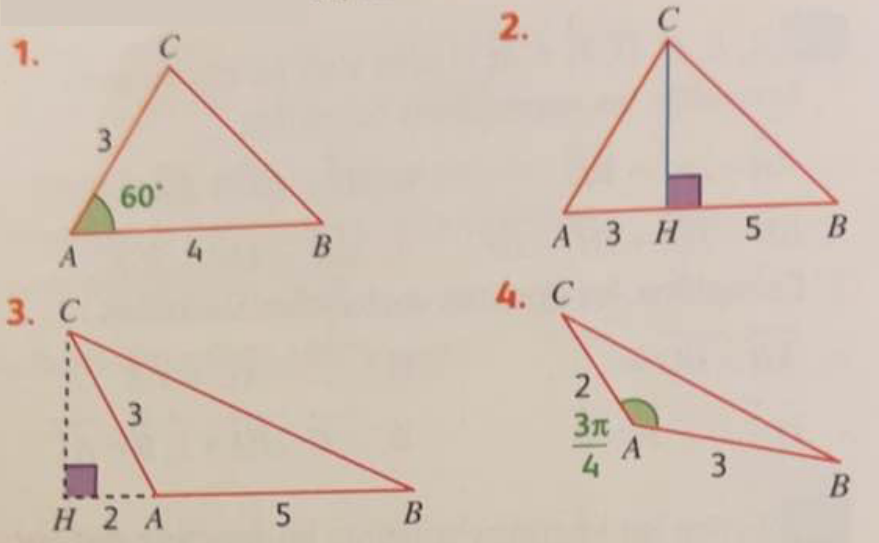
\includegraphics[scale=0.4]{1.04.02-Img03}
\end{center}

\exercice{}

Dans chaque cas, calculer le produit scalaire $\vv{u} \cdot \vv{v}$.
\begin{enumMet}
	\item $\vv{u}(1 ; 2)$ et $\vv{v}(3 ;-1)$;
	\item $\vv{u}(-1 ; 3)$ et $\vv{v}(12 ; 7)$;
	\item $\vv{u}\left(-\frac{11}{4} ;-15\right)$ et $\vv{v}\left(4 ;-\dfrac{2}{5}\right)$;
	\item $\vv{u}(-1+\sqrt{3} ;-3)$ et $\vv{v}(-1-\sqrt{3} ;-1)$.
\end{enumMet}

\exercice{}

On considère les points $\mathrm{A}(5 ;-3), \mathrm{B}(-2 ; 7), \mathrm{C}\left(\dfrac{-1}{2} ; 0\right)$ et $\mathrm{D}\left(-5 ; \dfrac{3}{4}\right)$. 

Calculer les produits scalaires $\vv{\mathrm{AB}} \cdot \vv{\mathrm{CD}}, \vv{\mathrm{AC}} \cdot \vv{\mathrm{BD}}$ et $\vv{\mathrm{AD}} \cdot \vv{\mathrm{BC}}$.

\exercice{}

Soit $\mathrm{A}, \mathrm{B}$ et C trois points du plan de coordonnées respectives: $(-4 ; 1),(-1 ; 2)$ et $(1 ;-4)$.
\begin{enumMet}
	\item Calculer $\vv{B A} \cdot \vv{B C}$.
	\item Quelle est la nature du triangle $A B C$ ?
\end{enumMet}

\exercice{}

Soit $A B C$ un triangle. Dans chaque cas, calculer la mesure en degré de l'angle $\widehat{B A C}$.
\begin{enumMet}
	\item $A B=3, A C=4$ et $\vv{A B} \cdot \vv{A C}=6 \sqrt{3}$.
	\item $A B=16, A C=48$ et $\vv{A B} \cdot \vv{A C}=-133$.
\end{enumMet}

On arrondira au degré près.

\exercice{}

Soit $A, B$ et $C$ trois points du plan de coordonnées respectives:

$(-5 ;-3),(-1 ;-6)$ et $(-5 ;-1)$.
\begin{enumMet}
	\item Calculer $\vv{C A} \cdot \vv{C B}$.
	\item En déduire $\widehat{B C A}$ en degré à $10^{-2}$ près.
\end{enumMet}

\exercice{}

Soit $A B C$ un triangle tel que $A B=\sqrt{13}, A C=\sqrt{5}$ et $\mathrm{BC}=\sqrt{10}$. 

Calculer $\vv{\mathrm{AB}} \cdot \vv{\mathrm{AC}}$ et $\vv{\mathrm{BA}} \cdot \vv{\mathrm{BC}}$.

\exercice{}

Soit $A B C$ un triangle tel que $A B=\dfrac{3}{2}, A C=6$ et $\mathrm{BC}=\dfrac{5}{2}$. Calculer $\vv{\mathrm{AB}} \cdot \vv{\mathrm{AC}}$.

\exercice{}

Soit $A B C$ un triangle tel que $A B=\sqrt{50}, A C=\sqrt{90}$ et $B C=\sqrt{41}$.
\begin{enumMet}
	\item \begin{enumMet}
		\item Calculer $\vv{A B} \cdot \vv{A C}$.
		\item En écrivant $\vv{A B} \cdot \vv{A C}$ en fonction du cosinus, déduire une valeur approchée en degré à $10^{-1}$ près de l'angle $\widehat{B A C}$.
	\end{enumMet}
	\item Calculer les valeurs approchées à $10^{-1}$ près des autres angles du triangle $A B C$.
\end{enumMet}


\exercice{ - Ex 48 p 253}

Soit le triangle $A B C$ tel que $A B=10, A C=16$ et $B C=8$ et soit les points $M$ et $N$ tels que $\vv{A M}=\dfrac{3}{5} \vv{A B}$ et $\vv{\mathrm{AN}}=\dfrac{1}{4} \vv{\mathrm{AC}}$

\begin{center}
	\begin{tikzpicture}[general, scale=0.5]
		\draw [quadrillage] (-1,-1) grid (17,8);
		\draw[color=Noir, epais] (0,0)--(8,6)--(15.61,3.52)--cycle;
		\point{0}{0}{A}{left}
		\point{8}{6}{B}{above}
		\point{15.61}{3.52}{C}{right}
		\pointFigure{4.8}{3.6}{M}{above left}
		\pointFigure{3.9}{0.88}{N}{above left}
		\draw [shift={(5.826532468208898,6.707480518578612)},line width=0.5mm,color=ForestGreen,fill=ForestGreen,fill opacity=0.10000000149011612] (0,0) -- (-108.28057787951006:0.6) arc (-108.28057787951006:-18.030470158762476:0.6) -- cycle;
		\draw [color=Noir, epais] (3.90,0.88)-- (5.83,6.71);
		\draw [color=Noir, epais] (15.61,3.52)-- (5.83,6.71);
		\draw[color=ForestGreen] (6.14,7.21) node {$(\vv{MN}, \vv{BC})$};
	\end{tikzpicture}
\end{center}

\begin{enumMet}
	\item Calculer $\vv{MN} \cdot \vv{BC}$.
%	\begin{corrBox}
%		$\vv{MN} \cdot \vv{BC}=\left(\vv{MA}+\vv{AN}\right)\cdot\vv{BC}$\\
%		$\phantom{\vv{MN} \cdot \vv{BC}}=\left(-\dfrac{3}{5}\vv{AB}+\dfrac{1}{4}\vv{AC}\right)\cdot\vv{BC}$\\
%		$\phantom{\vv{MN} \cdot \vv{BC}}=-\dfrac{3}{5}\vv{AB}\cdot\vv{BC}+\dfrac{1}{4}\vv{AC}\cdot\vv{BC}=\dfrac{3}{5}\vv{BA}\cdot\vv{BC}+\dfrac{1}{4}\vv{CA}\cdot\vv{CB}$\\
%		$\phantom{\vv{MN} \cdot \vv{BC}}=\dfrac{3}{5}\left(\dfrac{1}{2}(AB^2+BC^2-AC^2)\right)+\dfrac{1}{4}\left(\dfrac{1}{2}(AC^2+BC^2-AB^2)\right)$\\
%		$\phantom{\vv{MN} \cdot \vv{BC}}=\dfrac{3}{10}\left(10^2+8^2-16^2\right)+\dfrac{1}{8}\times \left(16^2+8^2-10^2\right)$\\
%		$\phantom{\vv{MN} \cdot \vv{BC}}=-\dfrac{1}{10}=-0,1$	
%	\end{corrBox}
	\item Calculer $\mathrm{MN}^2$.
%	\begin{corrBox}
%		$MN^2=\vv{MN} \cdot \vv{MN}=\left(\vv{MA}+\vv{AN}\right)\cdot\left(\vv{MA}+\vv{AN}\right)$\\
%		$\phantom{MN^2=\vv{MN} \cdot \vv{MN}}=\left(-\dfrac{3}{5}\vv{AB}+\dfrac{1}{4}\vv{AC}\right)\cdot\left(-\dfrac{3}{5}\vv{AB}+\dfrac{1}{4}\vv{AC}\right)$\\
%		$\phantom{MN^2=\vv{MN} \cdot \vv{MN}}=\dfrac{9}{25}\vv{AB}\cdot\vv{A B}-\dfrac{3}{10}\vv{A B}\cdot\vv{AC}+\dfrac{1}{16}\vv{AC}\cdot\vv{AC}$\\
%		$\phantom{MN^2=\vv{MN} \cdot \vv{MN}}=\dfrac{9}{25}\times AB^2-\dfrac{3}{20}(AB^2+AC^2-BC^2)+\dfrac{1}{16}\times AC^2$\\
%		$\phantom{MN^2=\vv{MN} \cdot \vv{MN}}=\dfrac{9}{25}\times 10^2-\dfrac{3}{20}(10^2+16^2-8^2)+\dfrac{1}{16}\times 16^2$\\
%		$\phantom{MN^2=\vv{MN} \cdot \vv{MN}}=\dfrac{41}{5}=8,2$
%		
%	\end{corrBox}
	\item En déduire une valeur approchée en degré à $10^{-1}$ près de l'angle géométrique $|(\vv{\mathrm{MN}}, \vv{\mathrm{BC}})|$.
%	\begin{corrBox}
%		On sait que $\vv{MN} \cdot \vv{BC}=-\dfrac{1}{10}=-0,1$ et que $\vv{MN} \cdot \vv{BC}=MN\times BC\times \cos(\vv{MN}, \vv{BC})$\\
%		D'ou : \\
%		$(\vv{MN}, \vv{BC})=\arccos\left(\dfrac{-0,1}{\sqrt{8,2}\times 8}\right)\approx90,25\degree$
%	\end{corrBox}
\end{enumMet}

\exercice{ - Ex 54 p 254}
Soit A, B, C trois points du plan de coordonnées respectives $(1 ; 5),(-7 ; 3),(0 ;-2)$ et soit I le milieu du segment $[A B]$.

Déterminer la valeur exacte de l'aire du triangle ACI.

%\begin{corrBox}
%	\begin{minipage}[c]{0.45\linewidth}
%		\begin{center}
%			\begin{tikzpicture}[general, scale=0.5]
%				\draw [quadrillage] (-8,-3) grid (2,6);
%				\axeOI{-8}{2}
%				\axeOJ{-3}{6}
%				\origineO
%				\point{1}{5}{A}{above}
%				\point{-7}{3}{B}{above}
%				\point{0}{-2}{C}{right}
%				\pointGraphique{-3}{4}{I}{above}
%				\draw[color=Noir, epais] (1,5)--(-7,3)--(0,-2)--cycle;
%				\draw[color=Noir, epais] (-3,4)--(0,-2);
%				\draw[line width=0.5mm,color=ForestGreen,fill=ForestGreen,fill opacity=0.1] (0.36,3.52) -- (0.3,3.1) -- (0.72,3.04) -- (0.78,3.46) -- cycle; 
%				\draw [color=ForestGreen, epais,dash pattern=on 5pt off 5pt] (-3.,4.)-- (0.78,3.46);
%				\point{0.78}{3.46}{H}{right}
%			\end{tikzpicture}
%		\end{center}
%	\end{minipage} \hfill
%	\begin{minipage}[c]{0.45\linewidth}
%		L'aire du triangle ACI est $\EuScript{A}=\dfrac{AC\times IH}{2}$ or dans le triangle rectangle AIH, on a :
%		
%		$IH=AI\times \sin\left(\widehat{BAC}\right)$ donc l'aire du triangle ACI est $\EuScript{A}=\dfrac{AC\times AI\times \sin\left(\widehat{BAC}\right)}{2}$	
%		
%		On calcule l'angle $\widehat{BAC}$ à l'aide du produit scalaire $\vv{AI}\cdot\vv{AC}$:	
%	\end{minipage}
%	Le point I a pour coordonnées : $I\left(\dfrac{x_A+x_B}{2};\dfrac{y_A+y_B}{2}\right)$ soit $I(-3;4)$.\\
%	$\Coord{AI}{x_I-x_A}{y_I-y_A}=\Coord{AI}{-3-1}{4-5}=\Coord{AI}{-4}{-1} \Longrightarrow AI=\sqrt{(-4)^2+(-1)^2}=\sqrt{17}$\\
%	$\Coord{AC}{x_C-x_A}{y_C-y_A}=\Coord{AC}{0-1}{-2-5}=\Coord{AC}{-1}{-7} \Longrightarrow AC=\sqrt{(-1)^2+(-7)^2}=\sqrt{50}$\\
%	D'une part : $\vv{AI}\cdot\vv{AC}=-4\times (-1)+(-1)\times (-7)=11$ et d'autre part:\\
%	$\vv{AI}\cdot\vv{AC}=AI\times AC\times \cos\left(\widehat{BAC}\right) = \sqrt{17}\times \sqrt{50}\times \cos\left(\widehat{BAC}\right)$.\\
%	On a donc $\widehat{BAC}=\arccos\left(\dfrac{11}{\sqrt{17}\times \sqrt{50}}\right)\approx67,8\degree$\quad \quad Finalement : \\
%	$\EuScript{A}=\dfrac{AC\times AI\times \sin\left(\widehat{BAC}\right)}{2}=\dfrac{\sqrt{50}\times \sqrt{17}\times \sin\left(\arccos\left(\dfrac{11}{\sqrt{17}\times \sqrt{50}}\right)\right)}{2}=\dfrac{27}{2}=13,5$
%	
%\end{corrBox}


\exercice{ - Ex 55 p 254}
Soit A, B, C, D quatre points du plan de coordonnées respectives: $(-3 ; 3),(2 ; 5),(6 ; 0)$ et $(1 ;-2)$.
\begin{enumMet}
	\item Démontrer que le quadrilatère $A B C D$ est un parallélogramme.
%	\begin{corrBox}
%		\begin{minipage}[c]{0.45\linewidth}
%			$\Coord{AB}{x_B-x_A}{y_B-y_A}=\Coord{AB}{2-(-3)}{5-3}=\Coord{AB}{5}{2}$\\
%			$\Coord{DC}{x_C-x_D}{y_C-y_D}=\Coord{DC}{6-1}{0-(-2)}=\Coord{DC}{5}{2}$\\
%			On a $\vv{AB}=\vv{DC}$ donc d'après la règle du parallélogramme, ABCD est un parallélogramme.
%		\end{minipage} \hfill
%		\begin{minipage}[c]{0.45\linewidth}
%			\begin{center}
%				\begin{tikzpicture}[general, scale=0.5]
%					\draw [quadrillage] (-4,-3) grid (7,6);
%					\axeOI{-4}{7}
%					\axeOJ{-3}{6}
%					\origineO
%					\point{-3}{3}{A}{above left}
%					\point{2}{5}{B}{right}
%					\point{6}{0}{C}{above right}
%					\point{1}{-2}{D}{below right}
%					\draw[color=Noir, epais] (-3,3)--(2,5)--(6,0)--(1,-2)--cycle;
%					\draw[epais,color=ForestGreen,fill=ForestGreen,fill opacity=0.1] (-1.69,2.05) -- (-1.96,2.38) -- (-2.29,2.11) -- (-2.02,1.78) -- cycle; 
%					\draw [color=ForestGreen, epais,dash pattern=on 5pt off 5pt] (2.,5.)-- (-2.02,1.78);
%					\point{-2.02}{1.78}{H}{below left}	
%				\end{tikzpicture}
%			\end{center}
%		\end{minipage}
%		
%	\end{corrBox}
	\item Déterminer une valeur approchée de l'aire de $A B C D$ à $10^{-2}$ près.
%	\begin{corrBox}
%		L'aire du parallélogramme est $\EuScript{A}=HB\times AD$ or dans le triangle rectangle ABH, on a :
%		
%		$HB=AB\times \sin\left(\widehat{BAD}\right)$ donc l'aire du parallélogramme est $A=AD\times AB\times \sin\left(\widehat{BAD}\right)$	
%		
%		On calcule l'angle $\widehat{BAD}$ à l'aide du produit scalaire $\vv{AD}\cdot\vv{AB}$:
%		$\Coord{AD}{x_D-x_A}{y_D-y_A}=\Coord{AD}{1-(-3)}{-2-3}=\Coord{AD}{4}{-5}$\\
%		$\vv{AD}\cdot\vv{AB}=5\times 4+2\times (-5)=10$\\
%		On a $AD= \sqrt{4^2+(-5)^2}=\sqrt{41}$ et $AB= \sqrt{5^2+2^2}=\sqrt{29}$ \\
%		D'autre part $\vv{AD}\cdot\vv{AB}=AD\times AB\times \cos\left(\widehat{BAD}\right)=\sqrt{41}\times \sqrt{29}\times \cos\left(\widehat{BAD}\right)$\\
%		Donc $10=\sqrt{41}\times \sqrt{29}\times \cos\left(\widehat{BAD}\right) \iff \widehat{BAD} = \arccos\left(\dfrac{10}{\sqrt{41}\times \sqrt{29}}\right)\approx73,14\degree$\\
%		\ \\
%		$\EuScript{A}=AD\times AB\times \sin\left(\widehat{BAD}\right)=\sqrt{41}\times \sqrt{29}\times \sin\left(\arccos\left(\dfrac{10}{\sqrt{41}\times \sqrt{29}}\right)\right)=33$
%	\end{corrBox}
\end{enumMet}

\exercice{ - Ex 70 p 255}

Dans un jeu vidéo, Super Ninja court pour échapper à ses ennemis. Il arrive au bord d'une rivière de 7 mètres de large et aperçoit un rocher triangulaire sur l'autre rive. Vite ! Super Ninja doit couper un arbre pour traverser la rivière en le posant sur la pointe du rocher. Mais quelle longueur doit avoir au minimum son arbre? Heureusement que Super Ninja connaît les dimensions (en mètre) du rocher...

En utilisant les données de la figure ci-dessous, calculer SC. On arrondira au mètre près.
\begin{center}
	\definecolor{zzttqq}{rgb}{0.6,0.2,0.}
	\definecolor{qqqqff}{rgb}{0.,0.,1.}
	\definecolor{wqwqwq}{rgb}{0.376,0.376,0.376}
	\begin{tikzpicture}[line cap=round,line join=round,>=triangle 45,x=1.0cm,y=1.0cm]
		\draw [line width=2.pt,color=wqwqwq] (2.,1.)-- (4.8,1.);
		\draw [line width=2pt,dash pattern=on 5pt off 5pt,color=qqqqff] (4.8,1.)-- (11.8,1.);
		\draw [line width=2.pt,color=wqwqwq] (2.,1.)-- (3.64,2.75);
		\draw [line width=2.pt,color=wqwqwq] (3.64,2.75)-- (4.8,1.);
		\draw [line width=2.8pt,color=zzttqq] (11.8,1.)-- (2,3.1);
		\draw [line width=2.8pt,color=zzttqq] (2,3.1)-- (1.4,4.1);
		\draw [line width=2.8pt,color=zzttqq] (2,3.1)-- (1,3.7);
		\draw [line width=2.8pt,color=zzttqq] (2,3.1)-- (1.,3.);
		\draw [line width=2.8pt,color=zzttqq] (2,3.1)-- (1,2.5);
		\draw (1.6,1.1) node {$A$};
		\draw (4.94,1.2) node {$B$};
		\draw (3.22,0.7) node {$2,8$};
		\draw (11.9,1.3) node {$S$};
		\draw (7.88,0.7) node {$7$};
		\draw (3.78,3.) node {$C$};
		\draw (2.5,2.11) node {$2,4$};
		\draw (4.56,2.01) node {$2,1$};
	\end{tikzpicture}
\end{center}
%\begin{corrBox}
%	\grasInMet{Dans le triangle BAC, on calcule l'angle $\widehat{BAC}$ à l'aide du produit scalaire.}
%	
%	$\vv{AB}\cdot\vv{AC}=\dfrac{1}{2}\left(AB^2+AC^2-BC^2\right)=\dfrac{1}{2}\left(2,8^2+2,4^2-2,1^2\right)=4,595$
%	
%	D'autre part : $\vv{AB}\cdot\vv{AC}=AB\times AC\times \cos\left(\widehat{BAC}\right)=2,8\times 2,4\times \cos\left(\widehat{BAC}\right)$
%	
%	d'où : $4,595=2,8\times 2,4\times \cos\left(\widehat{BAC}\right) \iff \cos\left(\widehat{BAC}\right)=\dfrac{4,595}{2,8\times 2,4}=\dfrac{919}{1344}$
%	
%	\grasInMet{On se place maintenant dans le triangle ASC}
%	
%	$\vv{AS}\cdot\vv{AC}=AS\times AC\times \cos\left(\widehat{BAC}\right)=9,8\times 2,4\times \dfrac{919}{1344}=\dfrac{6433}{400}$
%	
%	D'autre part : $\vv{AS}\cdot\vv{AC}=\dfrac{1}{2}\left(AS^2+AC^2-SC^2\right)=\dfrac{1}{2}\left(9,8^2+2,4^2-SC^2\right)$
%	
%	d'où : 
%	\begin{align*}
%		& \dfrac{6433}{400}=\dfrac{1}{2}\left(9,8^2+2,4^2-SC^2\right)\\
%		\iff & \dfrac{6433}{200}=9,8^2+2,4^2-SC^2\\
%		\iff & SC^2=9,8^2+2,4^2-\dfrac{6433}{200}\\
%		\iff & SC^2=69,635\\
%		\iff & SC=\sqrt{69,635}\approx8,34m
%	\end{align*}
%	
%	
%\end{corrBox}
\end{document}

